\chapter{Teoría de Promediación}

El análisis de sistemas no lineales con comportamientos oscilatorios puede ser extremadamente desafiante debido a la interacción entre términos no lineales y oscilaciones rápidas. En muchos casos, los métodos analíticos tradicionales fallan o resultan inmanejables, mientras que los métodos numéricos pueden ser costosos computacionalmente o poco precisos. La teoría de promediación aborda estos problemas al transformar las ecuaciones originales en un sistema equivalente más simple que describe el comportamiento medio del sistema \cite{hinch1991perturbation}.

Esta aproximación es particularmente útil cuando los parámetros del sistema están sujetos a pequeñas perturbaciones, lo que permite capturar la dinámica esencial sin perder información crítica sobre los ciclos límite o comportamientos oscilatorios \cite{bender2013advanced}.

\section{Teoría de perturbaciones}

Definimos un \textbf{problema perturbado} como una ecuación 

\begin{equation}\label{eq: problemaPerturbado}
	P^\epsilon\left(x\right)=0
\end{equation}

que incluye un parámetro pequeño $\epsilon$ con $0<\epsilon<1$, el cual que representa la perturbación.\\

El objetivo es encontrar soluciones aproximadas $x=x\left(\epsilon\right)$ en función de este parámetro y estudiar su comportamiento cuando $\epsilon\to0$ \cite{hinch1991perturbation}.\\

Para estudiar el comportamiento asintótico de las soluciones vamos a introducir el concepto de función de orden.

\begin{definition}[Función de orden]
	Se dice que una función $\delta=\delta\left(\epsilon\right)$ es de orden si cumple las siguientes condiciones:
	\begin{enumerate}
		\item Es continua en una vecindad de $\epsilon=0$.
		\item Tiene signo definido en esa vecindad (es decir, $\delta(\epsilon)>0$ o $\delta(\epsilon)<0$ para $0<\epsilon<\epsilon_0$ con $\epsilon_0>0$).
		\item Existe el límite:
		$$\displaystyle\lim_{\epsilon\to0}\delta\left(\epsilon\right)$$
	\end{enumerate}
\end{definition}

\begin{definition}
	Sean $\delta_1\left(\epsilon\right)$ y $\delta_2\left(\epsilon\right)$ funciones de orden. Decimos que: 
	\begin{enumerate}
		\item $\delta_1\left(\epsilon\right)=O\left(\delta_2\left(\epsilon\right)\right)$ si existe $k\in\mathbb{R}^+$ y un $\epsilon_0>0$ tales que:
		\begin{equation}\label{eq: Big-O}
			|\delta_1\left(\epsilon\right)|\leq k|\delta_2\left(\epsilon\right)|
		\end{equation}
		para todo $0<\epsilon<\epsilon_0$.\\

		Esta definición describe una cota superior en el crecimiento de la función $\delta_1\left(\epsilon\right)$ en términos de $\delta_2\left(\epsilon\right)$ cuando $\epsilon\to0$. Es decir, $\delta_2(\epsilon)$ actúa como una cota superior para $\delta_1(\epsilon)$ \cite{bender2013advanced}.\\
		\item $\delta_1\left(\epsilon\right)=o(\delta_2\left(\epsilon\right))$ si:
		\begin{equation}\label{eq: small-o}
		\displaystyle\lim_{\epsilon\to0}\frac{\delta_1\left(\epsilon\right)}{\delta_2\left(\epsilon\right)}=0
		\end{equation}
		Esta definición indica que $\delta_1\left(\epsilon\right)$ es asintóticamente insignificante en comparación con $\delta_2\left(\epsilon\right)$ cuando $\epsilon\to0$; es decir, $\delta_2(\epsilon)$ crece (o decrece) más rápido que $\delta_1(\epsilon)$ \cite{bender2013advanced}.\\
	\end{enumerate}
\end{definition} 

Consideremos las funciones $\delta_1\left(\epsilon\right)=\ln\left(1+\epsilon\right)$ y $\delta_2\left(\epsilon\right)=\epsilon$.\\

La serie de Taylor de $\ln\left(1+\epsilon\right)$ alrededor de $\epsilon=0$ es:

$$\ln\left(1+\epsilon\right)=\epsilon-\frac{\epsilon^2}{2}+\frac{\epsilon^3}{3}-\dots$$

evaluamos el límite:

$$\displaystyle\lim_{\epsilon\to0}\frac{\delta_1\left(\epsilon\right)}{\delta_2\left(\epsilon\right)}=\lim_{\epsilon\to0}\frac{\epsilon-\frac{\epsilon^2}{2}+\frac{\epsilon^3}{3}-\dots}{\epsilon}=\lim_{\epsilon\to0}\left(1-\frac{\epsilon}{2}+\frac{\epsilon^2}{3}-\dots\right)=1.$$

El límite es distinto de cero, por lo que $\ln\left(1+\epsilon\right)$ no es $o\left(\epsilon\right)$. Sin embargo, dado que el límite es finito y positivo, concluimos que $\ln\left(1+\epsilon\right)=O\left(\epsilon\right)$ \cite{bender2013advanced}.\\

Veamos algunos ejemplos más para comprender mejor estas definiciones.

\begin{example}
    
    Sea \(\delta_1(\epsilon) = \sin(\epsilon)\) y \(\delta_2(\epsilon) = \epsilon\).

    Sabemos que para \(\epsilon \to 0\):
    
    \[
    \sin(\epsilon) = \epsilon - \frac{\epsilon^3}{6} + \frac{\epsilon^5}{120} - \dots
    \]
    
    Calculamos el límite:
    
    \[
    \lim_{\epsilon \to 0} \frac{\sin(\epsilon)}{\epsilon} = \lim_{\epsilon \to 0} \left(1 - \frac{\epsilon^2}{6} + \frac{\epsilon^4}{120} - \dots \right) = 1.
    \]
    
    El límite es finito y positivo, por lo que \(\sin(\epsilon) = O\left( \epsilon \right)\).
    
\end{example}

\begin{example}
    Sea \(\delta_1(\epsilon) = e^\epsilon - 1\) y \(\delta_2(\epsilon) = \epsilon\).

La serie de Taylor de \(e^\epsilon\) es:

\[
e^\epsilon = 1 + \epsilon + \frac{\epsilon^2}{2} + \frac{\epsilon^3}{6} + \dots
\]

Entonces:

\[
e^\epsilon - 1 = \epsilon + \frac{\epsilon^2}{2} + \frac{\epsilon^3}{6} + \dots
\]

Calculamos el límite:

\[
\lim_{\epsilon \to 0} \frac{e^\epsilon - 1}{\epsilon} = \lim_{\epsilon \to 0} \left(1 + \frac{\epsilon}{2} + \frac{\epsilon^2}{6} + \dots \right) = 1.
\]

Por lo tanto, \(e^\epsilon - 1 = O\left( \epsilon \right)\).

\end{example}

\begin{example}
    Sea \(\delta_1(\epsilon) = \epsilon^2\) y \(\delta_2(\epsilon) = \epsilon\).

Calculamos el límite:

\[
\lim_{\epsilon \to 0} \frac{\epsilon^2}{\epsilon} = \lim_{\epsilon \to 0} \epsilon = 0.
\]

Entonces, \(\epsilon^2 = o\left( \epsilon \right)\), lo que significa que \(\epsilon^2\) es insignificante en comparación con \(\epsilon\) cuando \(\epsilon \to 0\) \cite{bender2013advanced}.

\end{example}

\begin{example}
    Sea \(\delta_1(\epsilon) = \epsilon \ln(\epsilon)\) y \(\delta_2(\epsilon) = \epsilon\).

Para \(\epsilon \to 0^+\), \(\ln(\epsilon) \to -\infty\), por lo que \(\epsilon \ln(\epsilon) \to 0^-\).

Calculamos el límite:

\[
\lim_{\epsilon \to 0^+} \frac{\epsilon \ln(\epsilon)}{\epsilon} = \lim_{\epsilon \to 0^+} \ln(\epsilon) = -\infty.
\]

Aunque el límite es infinito negativo, observamos que \(\epsilon \ln(\epsilon)\) tiende a cero más lentamente que \(\epsilon\). Por lo tanto, \(\epsilon \ln(\epsilon) = o(1)\), pero no es \(o\left( \epsilon \right)\) ni \(O\left( \epsilon \right)\) \cite{bender2013advanced}.

\end{example}

\begin{example}
    Sea \(\delta_1(\epsilon) = e^{-1/\epsilon}\) y \(\delta_2(\epsilon) = \epsilon^n\) para cualquier \(n > 0\).

Cuando \(\epsilon \to 0^+\):

\[
e^{-1/\epsilon} \to e^{-\infty} = 0,
\]

y

\[
\lim_{\epsilon \to 0^+} \frac{e^{-1/\epsilon}}{\epsilon^n} = 0,
\]

ya que \(e^{-1/\epsilon}\) decrece más rápidamente que cualquier potencia de \(\epsilon\). Por lo tanto, \(e^{-1/\epsilon} = o\left( \epsilon^n \right)\) \cite{bender2013advanced}.

\end{example}

\begin{example}
    Sea \(\delta_1(\epsilon) = \epsilon^n\) y \(\delta_2(\epsilon) = e^{-1/\epsilon}\) para cualquier \(n > 0\).

Calculamos:

\[
\lim_{\epsilon \to 0^+} \frac{\epsilon^n}{e^{-1/\epsilon}} = \lim_{\epsilon \to 0^+} \epsilon^n e^{1/\epsilon} = \infty,
\]

ya que \(e^{1/\epsilon}\) crece más rápido que cualquier potencia negativa de \(\epsilon\). Por lo tanto, \(\delta_2(\epsilon) = o\left( \delta_1(\epsilon) \right)\) \cite{bender2013advanced}.

\end{example}

\section{Teoría de promediación}


Como vimos determinar la existencia y propiedades cualitativas y cuantitativas
de los ciclos límite en sistemas no lineales no es tarea fácil. En muchos
casos los métodos analíticos fallan o se vuelve sumamente complejo y los
métodos numéricos pueden ser ineficientes o inexactos. \\

El Método de Promediación es una herramienta poderosa y efectiva,
parte de la teoría de perturbaciones y nos ayuda a simplificar el análisis
de sistemas no lineales  transformando las ecuaciones originales en un sistema
más manejable. La premisa fundamental es que, bajo ciertas condiciones, el
comportamiento promedio del sistema a lo largo del tiempo puede revelar
la existencia y la estructura de los ciclos límite.\\

La aplicación del Método de Premediación para verificar la existencia de
ciclos límite en sistemas no lineales no solo proporciona una técnica
analítica robusta sino que también ofrece una perspectiva más profunda
del comportamiento oscilatorio inherente en dichos sistemas. Este enfoque
no solo permite simplificar las ecuaciones diferenciales originales, sino
también captar la esencia del comportamiento dinámico del sistema,
facilitando así la identificación y caracterización de ciclos límite.\\

Definiendo el promedio local de una función y algunas de sus propiedades.

\begin{definition}
	Sea $f:\mathbb{R}\times\mathbb{R}^p\to\mathbb{R}^n$ continua y $T>0$.
	Definimos:
	\[
		f_T(t,x)=\frac{1}{T}\int_{0}^{T}f(t+\tau,x)d\tau
	\]
	como el promedio local de $f$.
\end{definition}

La función $f_T(t,x)$ calcula el valor promedio de la función $f(t,x)$ 
respecto a la variable $t$ en el intervalo $[t,t+T]$, visto de otro 
modo, calcula el comportamiento promedio futuro del tiempo $t$ a tiempo $t+T$.

\begin{proposition}
	Sea $f:\mathbb{R}\times\mathbb{R}^p\to\mathbb{R}^n$ continua y de periodo $T$ en $t$, entonces
	\[
		f_T(t,x)=f_0(x)
	\]
\end{proposition}

Si la función a promediar es de Lipschitz entonces la diferencia entre ambas
funciones está acotada, esto quiere decri que el mapeo del promedio local de 
la función no se aleja demasiado de la función original, solo lo simplifica 
y guarda el comportamiento promedio de la función.
\begin{proposition}
	Si $\phi:\mathbb{R}\to\mathbb{R}$ es de Lipschitz en $\mathbb{R}$ con constante de Lipschitz $\lambda$ entonces
	\[
		|\phi(x)-\phi_T(x)|\leq\frac{\lambda T}{2}
	\]
	i.e. $\phi(t)$ es $o(T)$ con respecto a $\phi_T(x)$.
\end{proposition}

\begin{example}
	Consideremos la función $\phi(t)=\sqrt{t^2+1}$, esta función es de Lipschitz
	con constante $\lambda=1$, calculamos su promedio local con $T=0.5$

	$$\phi_T(t)=\frac{1}{2T}(((T + t)\sqrt{1 + (T + t)^2} + \sinh^{-1}(T + t)) - (t\sqrt{1 + t^2} + \sinh^{-1}(t)))$$

	graficamos ambas funciones.

	\begin{figure}[h]
		\centering
		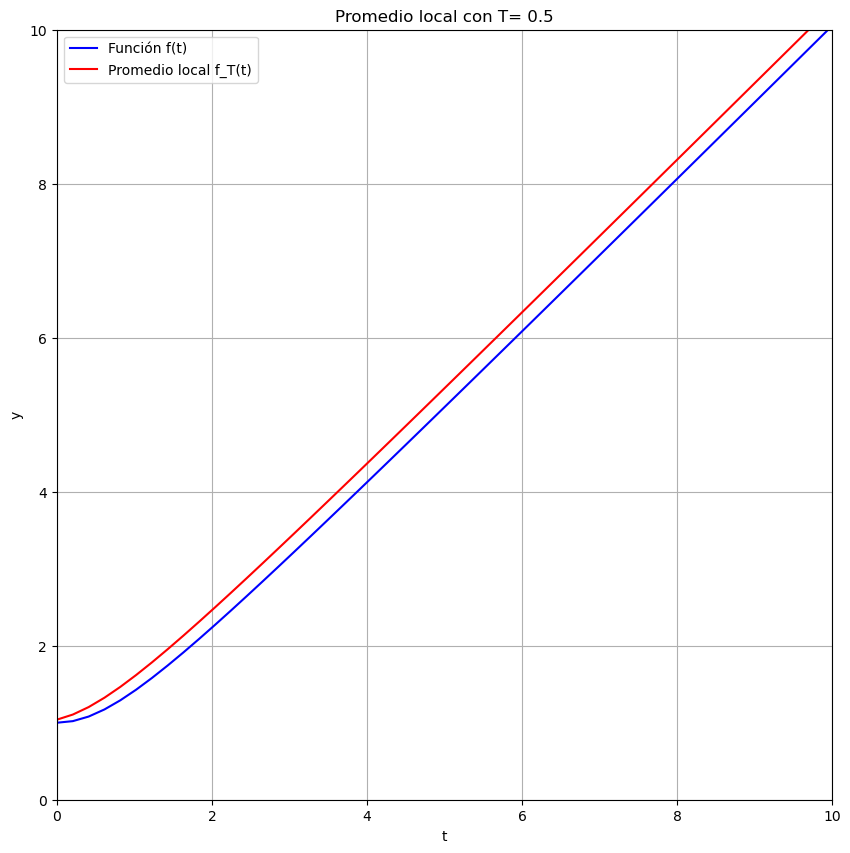
\includegraphics[width=10cm]{fl.png}
		\caption{Función vs  función promediada.}
	\end{figure}

	la diferencia esta acotada por $M=\frac{\lambda T}{2}=\frac{0.5}{2}=0.25$. En este caso en la
	gráfica se puede observar que la diferencia converge a la cota $M$.

	\begin{figure}[h]
		\centering
		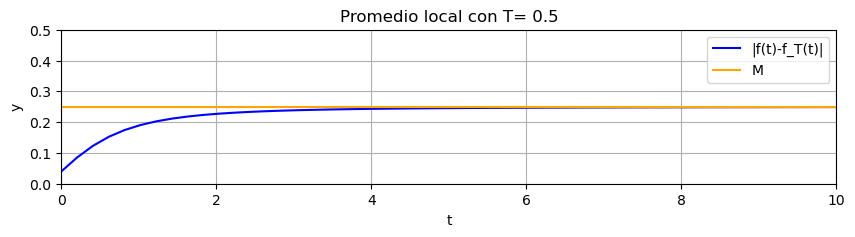
\includegraphics[width=13cm]{d.png}
		\caption{Diferencia de la Función con la función promediada.}
	\end{figure}

\end{example}

este comportamiento asintótico no necesariamente ocurre siempre, un ejemplo es la función $\sin(x)$. 

\begin{lemma}
	Consideremos la EDO
	\[
		x'=\epsilon f(t,x)
	\]
	con $x(0)=x_0$, donde $f$ es de Lipschitz en $x\in D\subseteq\mathbb{R}^n$
	y $f$ continua en $t\in[0,t]$.\\
	Sea $M=\sup_{x\in D} \sup_{0\leq\epsilon t\leq L} \left|f(t,x)\right|<+\infty$

	Si $\phi(t)=\int_{0}^{t}f(\tau,x(\tau))d\tau$ con $x$ solución de la EDO.
	\\Entonces:
	\[
		|\phi_T(t)-\int_{0}^{t}f_T(\tau,x(\tau))d\tau|\leq\frac{1}{2}(1+\lambda L)MT
	\]
	para $o(\frac{1}{\epsilon})=t$, donde $\lambda\equiv cte$ de Lipschitz.
	\\i.e. $\phi_T(t)=\int_{0}^{t}f_T(\tau,x(\tau))d\tau+o(T)$
\end{lemma}

\begin{lemma}
	Consideremos el problema de valor inicial
	\[
		x'=\epsilon f(t,x)
	\]
	$x(0)=x_0$, con $f$ Lipschitz en $x\in D\subseteq\mathbb{R}^n$ y continua
	en $t\in[0,t]$.

	Si $y$ es solución de 

	\begin{equation}
		y'=\epsilon f_T(t,y)
	\end{equation}
	
	, $y(0)=x_0$, entonces
	\[
		x(t)-y(t)=o(\epsilon T)
	\]
	p.t. $t=o(\frac{1}{\epsilon})$
\end{lemma}

\begin{theorem}\label{teorema: promedio}
	Consideremos $x'=\epsilon f(t,x)$, $x(t_0)=x_0$ y $y'=f^0(y)$, $y(t_0)=x_0$,
	donde $x_0,x,y\in D\subseteq\mathbb{R}^n$ y $\epsilon\in[0,\epsilon_0]$.\\

	Satisfaciendo:
	\begin{enumerate}
		\item $\bar{f}(t,x)$ es $T$ periódica con promedio $f^0(x)$.
		\item $f$ es continua en $t$ y Lipschitz en $x\in D$.
		\item $y(t)$ permanece en el interior de $D$ para todo $t=O(\frac{1}{\epsilon})$.
	\end{enumerate}
	Entonces
	\[x(t)-y(t)=O(\delta(\epsilon))\]
	para todo $t=o(\frac{1}{\epsilon})$ con $\delta=\delta(\epsilon)$ función de orden.
\end{theorem}

\section{Teoría del Promedio aplicado al 16 Problema de Hilbert}

Consideremos el sistema de ecuaciones en el plano polinomial de grado $n$ \eqref{eq: 16Hilbert}. Podemos reescribir el sistema como:

\begin{equation}\label{eq: 16Hilbertprom}
	y'= -x + \epsilon P(x,y)
	x'=y + \epsilon Q(x,y)
\end{equation}

Donde $P(x,y)$ y $Q(x,y)$ son polinomios de grado $2n$ de la forma:

\begin{equation}\label{eq: 16Hilbertprompol}
	\begin{matrix}
		P(x,y) = \sum_{i=0}^{n} \sum_{j=0}^{n} a_{i,j} x^i y^j \\
		Q(x,y) = \sum_{i=0}^{n} \sum_{j=0}^{n} b_{i,j} x^i y^j
	\end{matrix}
\end{equation}

Para poder aplicar el teorema \ref{teorema: promedio} debemos convertir el sistema \eqref{eq: 16Hilbertprom} a coordenadas polares.

Sustituimos \eqref{eq: 16Hilbertprom}, \eqref{eq: xpolar} y \eqref{eq: ypolar} en \eqref{es: drcart} y \eqref{eq: dthetacart}, obtenemos lo siguiente:

\[
 rr'=\epsilon r\cos(\theta)\sum_{i=0}^{n}\sum_{j=0}^{n}b_{i,j}r^{i+j}\cos(\theta)^i\sin(\theta)^j + \epsilon r\sin(\theta)\sum_{i=0}^{n}\sum_{j=0}^{n}a_{i,j}r^{i+j}\cos(\theta)^i\sin(\theta)^j
\]
\begin{equation}\label{eq: rpolhilbert}
 r'=\epsilon\sum_{i=0}^{n}\sum_{j=0}^{n}r^{i+j}(b_{i,j}\cos(\theta)^{i+1}\sin(\theta)^j+a_{i,j}\cos(\theta)^i\sin(\theta)^{j+1})
\end{equation}

Para $\theta$ tenemos:

\begin{equation}\label{eq: thetapolhilbert}
	r\theta'=\epsilon\sum_{i=0}^{n}\sum_{j=0}^{n}r^{i+j}(a_{i,j}\cos(\theta)^{i+1}\sin(\theta)^j-b_{i,j}\cos(\theta)^{i}\sin(\theta)^{j+1})+r
\end{equation}

Promediamos \eqref{eq: rpolhilbert}:

\[
\bar{r}'=\frac{1}{2\pi}\int_{0}^{2\pi}r'd\theta
\]

\[
\bar{r}'=\frac{1}{2\pi}\int_{0}^{2\pi}\epsilon\sum_{i=0}^{n}\sum_{j=0}^{n}r^{i+j}(b_{i,j}\cos(\theta)^{i+1}\sin(\theta)^j+a_{i,j}\cos(\theta)^i\sin(\theta)^{j+1})d\theta
\]

\[
\bar{r}'=\frac{\epsilon}{2\pi}\sum_{i=0}^{n}\sum_{j=0}^{n}r^{i+j}\left(b_{i,j}\int_{0}^{2\pi}\cos(\theta)^{i+1}\sin(\theta)^j d\theta+a_{i,j}\int_{0}^{2\pi}\cos(\theta)^i\sin(\theta)^{j+1} d\theta\right)
\]

por la ecuación \eqref{eq: integral_cos_sen_general_impar} tenemos:

\[
\bar{r}'=\frac{\epsilon}{2\pi}\sum_{i \text{ impar}}^{n}\sum_{j \text{ par}}^{n}r^{i+j}b_{i,j}\int_{0}^{2\pi}\cos(\theta)^{i+1}\sin(\theta)^j d\theta+\frac{\epsilon}{2\pi}\sum_{i \text{ par}}^{n}\sum_{j \text{ impar}}^{n}r^{i+j}a_{i,j}\int_{0}^{2\pi}\cos(\theta)^i\sin(\theta)^{j+1} d\theta
\]

Por la ecuación \eqref{eq: integral_cos_sen_general_pares} tenemos:

\begin{equation}\label{r_promedio}
	r'=\epsilon\sum_{i \text{ par}}^{n}\sum_{j \text{ par}}^{n}r^{i+j}\frac{b_{i,j}}{2^{i+j+1}}\frac{\left(i+1\right)!\left(j\right)!}{\left(\frac{i+1}{2}\right)!\left(\frac{j}{2}\right)!\left(\frac{i+j+1}{2}\right)!}+\epsilon\sum_{i \text{ impar}}^{n}\sum_{j \text{ impar}}^{n}r^{i+j}\frac{a_{i,j}}{2^{i+j+1}}\frac{\left(i!\right)\left(j+1\right)!}{\left(\frac{i}{2}\right)!\left(\frac{j+1}{2}\right)!\left(\frac{i+j+1}{2}\right)!}
\end{equation}

Notemos que al promediar solo se consideran del sistema \eqref{eq: 16Hilbertprompol}:
\begin{itemize}
	\item Para $x'$ los coeficientes $b_{i,j}$ con $i$ impar y $j$ par.
	\item Para $y'$ los coeficientes $a_{i,j}$ con $i$ par y $j$ impar.
\end{itemize}






	
\section{Ecuación de Van der Pol}
La ecuación del oscilador de Van der Pol describe el comportamiento de ciertos sistemas oscilantes no lineales.
Su fundamento físico se basa en el concepto de amortiguamiento no lineal y autodemostración de oscilaciones.
\begin{equation}\label{eq: VP}
	x''+x+\epsilon x'(x^2-1)=0
\end{equation}
donde $\epsilon$ es un parámetro de amortiguamiento no lineal.\\
\\El término $-\epsilon(1 - x^2)x'$ representa la no linealidad del amortiguamiento en el sistema. La expresión
$(1 - x^2)$ describe cómo el amortiguamiento varía en función de la posición del oscilador. Cuando $x$ es
pequeño, este término es cercano a $1$ y el amortiguamiento es lineal. Sin embargo, a medida que $x$
aumenta, el término $(1 - x^2)$ se hace más negativo, generando un efecto de amortiguamiento no lineal que
disminuye la velocidad del oscilador.\\
\\Extendemos a un sistema de ecuaciones.
\begin{equation}\label{eq: VPsis}
	\begin{matrix}
		y'=-x-\epsilon y(x^2-1) \\
		x'=y
	\end{matrix}
\end{equation}
Haremos el cambio de coordenadas a polares.
Sustituimos en $\eqref{eq: dxpolar}$ y $\eqref{eq: dypolar}$ en $\eqref{eq: VPsis}$
$$r\cos(\theta)\theta'+r'\sin(\theta)=-r\cos(\theta)-\epsilon r\sin(\theta)(r^2\cos^2(\theta)-1)$$
$$-r\sin(\theta)\theta'+r'\cos(\theta)=r\sin(theta)$$
entonces
\begin{equation}\label{eq: VPdr}
	r'=-\epsilon r\sin^2(\theta)(r^2\cos^2(\theta)-1)
\end{equation}
\begin{equation}\label{eq: VPdtheta}
	\theta'=-1-\epsilon r\sin(\theta)\cos(\theta)(r^2\cos(\theta^2)-1)
\end{equation}
Definimos para $\eqref{eq: VPdr}$ el promedio
\begin{equation}\label{eq: drbar}
	\bar{r}'=\bar{f}(\bar{r},\epsilon)
\end{equation}
donde
$$\bar{f}(\bar{r},\epsilon)=\frac{1}{2\pi}\int\limits_0^{2\pi}r'd\theta$$
Calculamos esta integral
$$\bar{f}(\bar{r},\epsilon)=\frac{1}{2\pi}\int\limits_0^{2\pi}-\epsilon r\sin^2(\theta)(r^2\cos^2(\theta)-1)d\theta$$
$$=\frac{1}{2\pi}[-\epsilon r^3\int\limits_0^{2\pi}\sin^2(\theta)\cos^2(\theta)d\theta+\epsilon r\int\limits_0^{2\pi}\sin^2(\theta)d\theta]$$
$$=\frac{1}{2\pi}[-\epsilon r^3[\frac{1}{32}(4\theta-\sin(4\theta))]_0^{2\pi}+\epsilon r[\frac{1}{2}(\theta-\sin(\theta)\cos(\theta))]_0^{2\pi}]$$
$$=\frac{1}{2\pi}[\frac{-\epsilon r^3}{32}(8\pi)+\frac{\epsilon r}{2}(2\pi)]=\frac{1}{2\pi}[\frac{-\epsilon r^3}{4}\pi+\epsilon r\pi].$$
Entonces
$$\bar{f}(\bar{r},\epsilon)=\frac{\epsilon r}{2}-\frac{\epsilon r^3}{8}$$
Promediamos $\theta$
$$\bar{\theta}=2\pi t$$
Vamos a analizar $\eqref{eq: drbar}$
\begin{equation}\label{eq: drvander}
	\bar{r}'=\frac{\epsilon}{8}r(4-r^2)
\end{equation}
\begin{figure}[h]
	\centering
	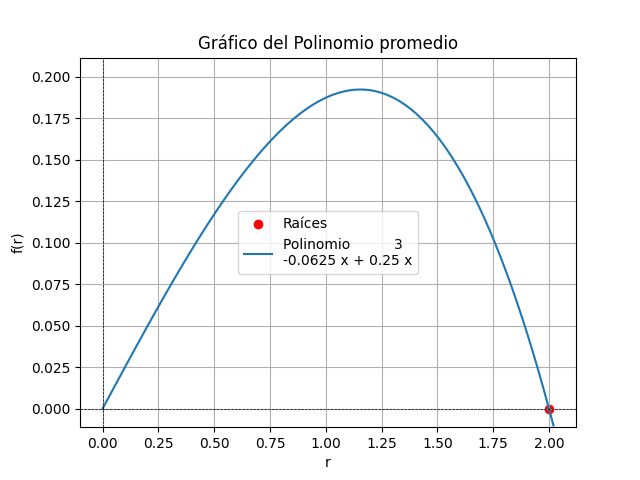
\includegraphics[width=14cm]{graficavanderpol.png}
	\caption{Plano fase de $\eqref{eq: drvander}$.}
\end{figure}
Las soluciones de equilibrio son $r=0$ y $r=2$.
\begin{enumerate}
	\item Si $0<r<2$, entonces $r'>0$, por lo que $0$ es un punto fuente o repulsivo.
	\item Si $r>2$, entonces $r'<0$, entonces $r=2$ es sumidero o atractor.
\end{enumerate}

\begin{figure}[h]
	\centering
	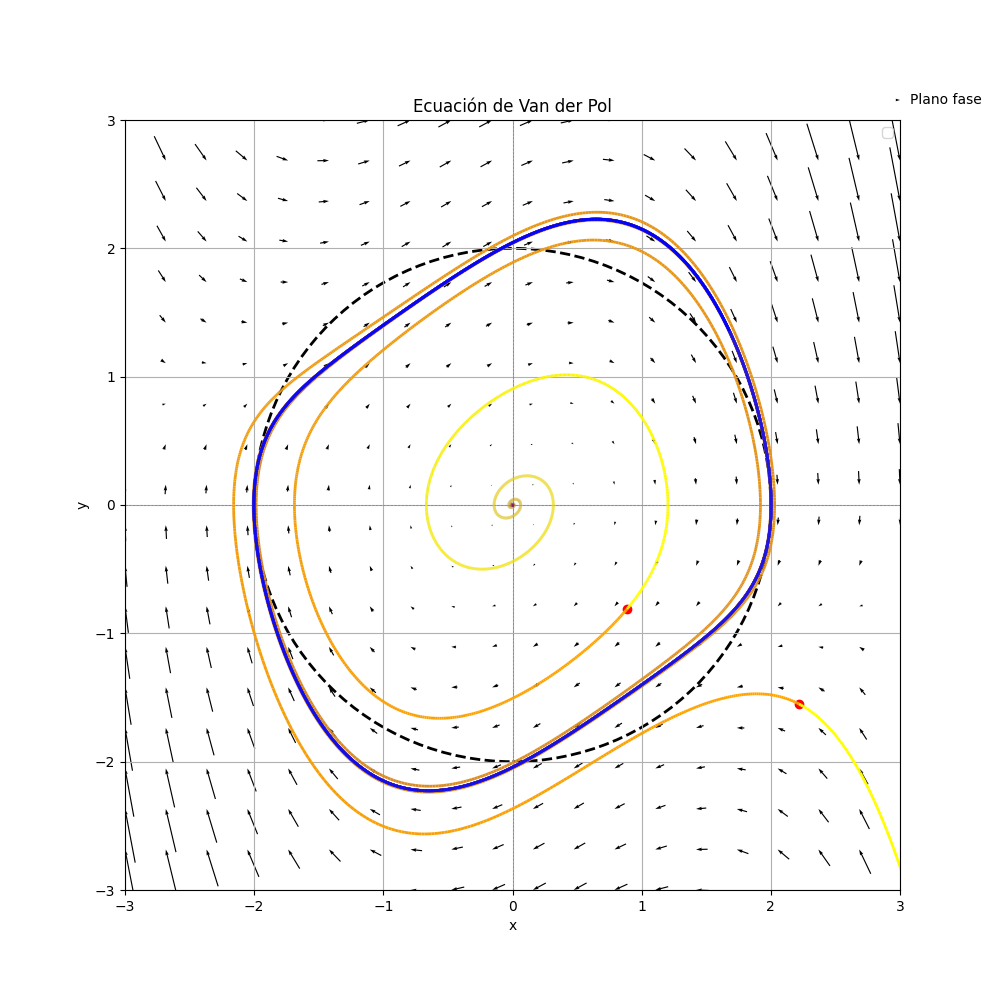
\includegraphics[width=11cm]{vanderpol.png}
	\caption{Plano fase. Dibujado en https://aeb019.hosted.uark.edu/pplane.html}
\end{figure}

Esto quiere decir que entre dos circunferencias de radios $0<r_{\min}<2$ y $2<r_{\max}$ existe al menos una curva cerrada a la cual las curvas convergen.

\section{Ecuación de Rayleigh}
La ecuación de Rayleigh con amortiguamiento no lineal, se utiliza
para estudiar oscilaciones no lineales en sistemas mecánicos y se encuentra en
diversos campos como la mecánica estructural y la dinámica de sistemas físicos.

$$x''+\epsilon(x'^2-1)x'+x=0$$

El parámetro $\epsilon$ es un coeficiente que controla la influencia del término no lineal en el amortiguamiento.
El término $\epsilon(x'^2 - 1)x'$ es el término no lineal en el amortiguamiento. Mientras que en el amortiguamiento
lineal la fuerza de amortiguamiento es proporcional a la velocidad, en este caso el amortiguamiento depende de
la velocidad al cuadrado y se modifica por el término $(x'^2 - 1)$. Esto introduce un comportamiento no lineal en e
l sistema y puede dar lugar a fenómenos como la autoexcitación y la respuesta no armónica.
Extendemos a un sistema de ecuaciones.

\begin{equation}\label{eq: Rayleigh}
	\begin{matrix}
		y'=-\epsilon(y^2-1)y-x \\
		x'=y
	\end{matrix}
\end{equation}
Haremos el cambio de coordenadas a polares.
$$r\cos(\theta)\theta'+r'\sin(\theta)=-\epsilon (r^2\sin^2(\theta)-1)r\sin(\theta)-\omega^2r\cos(\theta) $$
$$-r\sin(\theta)\theta'+r'\cos(\theta)=r\sin(\theta)$$
Obtenemos la ecuación.
\begin{equation}\label{eq: Rayleighpolar}
	r'=\epsilon(1-r^2\sin^2(\theta))r\sin^2(\theta)+r\sin(\theta)\cos(\theta)(1-\omega^2)
\end{equation}
Definimos para $\eqref{eq: Rayleighpolar}$ el promedio
$$\bar{r}=\bar{f}(\bar{r},\epsilon)=\frac{1}{2\pi}\int\limits_0^{2\pi}r'd\theta$$
Calculamos esta integral
$$\bar{f}(\bar{r},\epsilon)=\frac{1}{2\pi}\int\limits_0^{2\pi}[\epsilon(1-r^2\sin^2(\theta))r\sin^2(\theta)+r\sin(\theta)\cos(\theta)(1-\omega^2)]d\theta$$
$$=\frac{1}{2\pi}\epsilon r\int\limits_0^{2\pi}\sin^2(\theta)d\theta-\frac{1}{2\pi}\epsilon r^3\int\limits_0^{2\pi}\sin^4(\theta)d\theta+\frac{1}{2\pi}r(1-\omega^2)\int\limits_0^{2\pi}\cos(\theta)\sin(\theta)d\theta$$
$$=\frac{1}{2\pi}\epsilon r[\frac{1}{2}(\theta-\sin(\theta)\cos(\theta))]\Big|_2^{2\pi}-\frac{1}{2\pi}\epsilon r^3[\frac{1}{32}(-8\sin(2\theta)+\sin(4\theta)+12\theta)]\Big|_0^{2\pi}+$$
$$\frac{1}{2\pi}r(1-\omega^2)[\cos^2(\theta)]\Big|_0^{2\pi}]=\frac{1}{2\pi}\epsilon r\pi-\frac{1}{2\pi}\epsilon r^3\frac{3}{4}\pi$$
$$=\frac{\epsilon r}{8}(4-3r^2)$$
Entonces tenemos el sistema
$$\bar{r}'=\frac{\epsilon r}{8}(4-3r^2)$$
$$\bar{\theta}'=2\pi t$$
Las soluciones de equilibrio son $r=0$ y $r=\frac{2}{3}\sqrt{3}$
\begin{figure}[h]
	\centering
	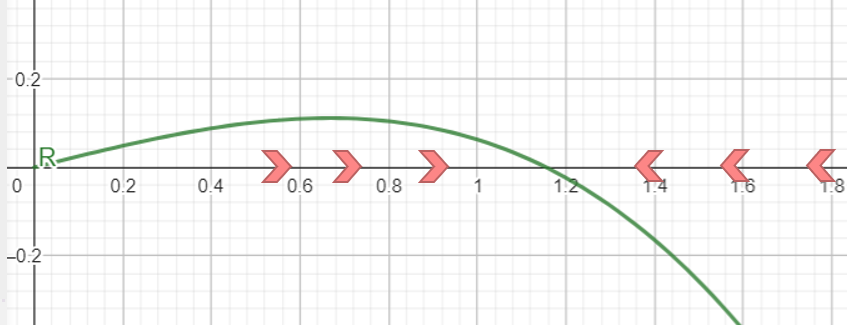
\includegraphics[width=9cm]{graficarayleigh.png}
	\caption{Plano fase.Dibujado en https://aeb019.hosted.uark.edu/pplane.html}
\end{figure}
\begin{figure}[h]
	\centering
	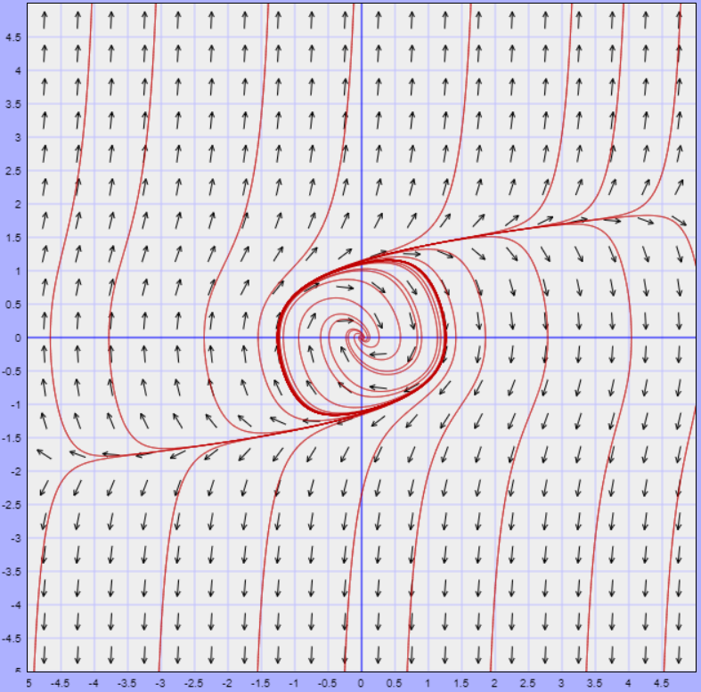
\includegraphics[width=11cm]{planorayleigh.png}
	\caption{Plano fase.Dibujado en https://aeb019.hosted.uark.edu/pplane.html}
\end{figure}
